%\titleformat*{\subsubsection}{\large\bfseries}

\section{Краткие теоретические сведения}
\subsection{Bluetooth}
Bluetooth\footnote{Bluetooth Technology Overview\href{https://www.bluetooth.com/learn-about-bluetooth/tech-overview/}{https://www.bluetooth.com/learn-about-bluetooth/tech-overview/}}
— это стандарт беспроводной технологии малого радиуса действия, который используется для обмена данными между стационарными и мобильными устройствами на коротких расстояниях с использованием радиоволн УВЧ в диапазонах ISM от 2,402 до 2,48 ГГц.
Он в основном используется в качестве альтернативы проводным соединениям, для обмена файлами между соседними портативными устройствами и подключения мобильных телефонов и музыкальных плееров с беспроводными наушниками.
В наиболее широко используемом режиме мощность передачи ограничена 2,5 мВт, что обеспечивает очень малую дальность до 10 метров


\subsection{Winsock2}
\quad {Для работы с внешними интерфейсами, в частности с bluetooth\footnote{Библиотека выступающая в качестве примера по подключению к Wiimote по bluetooth https://github.com/dolphin-emu/dolphin}, использовался Winsock2\footnote{Winsock2  \href{https://docs.microsoft.com/ru-ru/windows/win32/winsock/windows-sockets-start-page-2}{ https://docs.microsoft.com/ru-ru/windows/win32/winsock/windows-sockets-start-page-2}}}.\\
\quad Windows Sockets 2 \(Winsock\) позволяет программистам создавать расширенные приложения Интернета, интернет сети и другие сетевые приложения для передачи данных приложений по сети независимо от используемого сетевого протокола.

\par

\subsection{HID(Human Interface Device)}
\hypertarget{hid_theoretical_inf}{}

\quad \text{Для получения и передачи данных использовался HID}\\
\mbox{Устройства с HID-интерфейсом — это определение класса устройств}.
Использует универсальный драйвер USB для поддержки устройств HID, таких, как клавиатуры, мыши, игровые контроллеры и т.д.
До HID\footnote{Библиотека выбранная в качестве примера использования HID для работы с Wiimote https://github.com/wiiuse/wiiuse} устройства могли использовать только строго определенные протоколы для мышей и клавиатуры.\par
\quad {Для внедрения оборудования требуется либо перегрузить данные в существующий протокол}, либо создать нестандартное оборудование с собственным специализированным драйвером.
HID обеспечивает поддержку этих устройств "режима загрузки", добавляя поддержку инновационных инноваций с помощью расширяемых, стандартизированных и легко программируемых интерфейсов.


\subsection{Разработка с использованием продукции JetBrains и инструментов CMake}
\subsubsection{JetBrains}

\quad JetBrains\footnote{Документ рассказывающий о JetBrains и их продукции \\ \href{https://resources.jetbrains.com/storage/products/jetbrains/docs/corporate-overview/en-us/jetbrains_corporate_overview.pdf}{Jetbrains Corporation Overview PDF https://resources.jetbrains.com/storage/products/jetbrains/docs/corporate-overview/en-us/jetbrains\_corporate\_overview.pdf}}
- компания созданная тремя русскими разработчиками.
В данный момент специализирующаяся на создании инструментов для разработчиков программного обеспечения
Среди её IDE использовались Clion и IntelliJ Rust плагин\@.
\subsubsection{Clion}
\quad Clion\footnote{IDE от JetBrains предназначенная для разработки на языках C или C++.\href{ https://www.jetbrains.com/clion/}{https://www.jetbrains.com/clion/}}
- это IDE предназначенная для разработки на языках C или C++.
В неё включён пакте анализа кода, широкие возможности по генерации кода и перехода по нему в один клик.
Clion понимает современные стандарты C++ и обеспечивает поддержку предпроцессора.
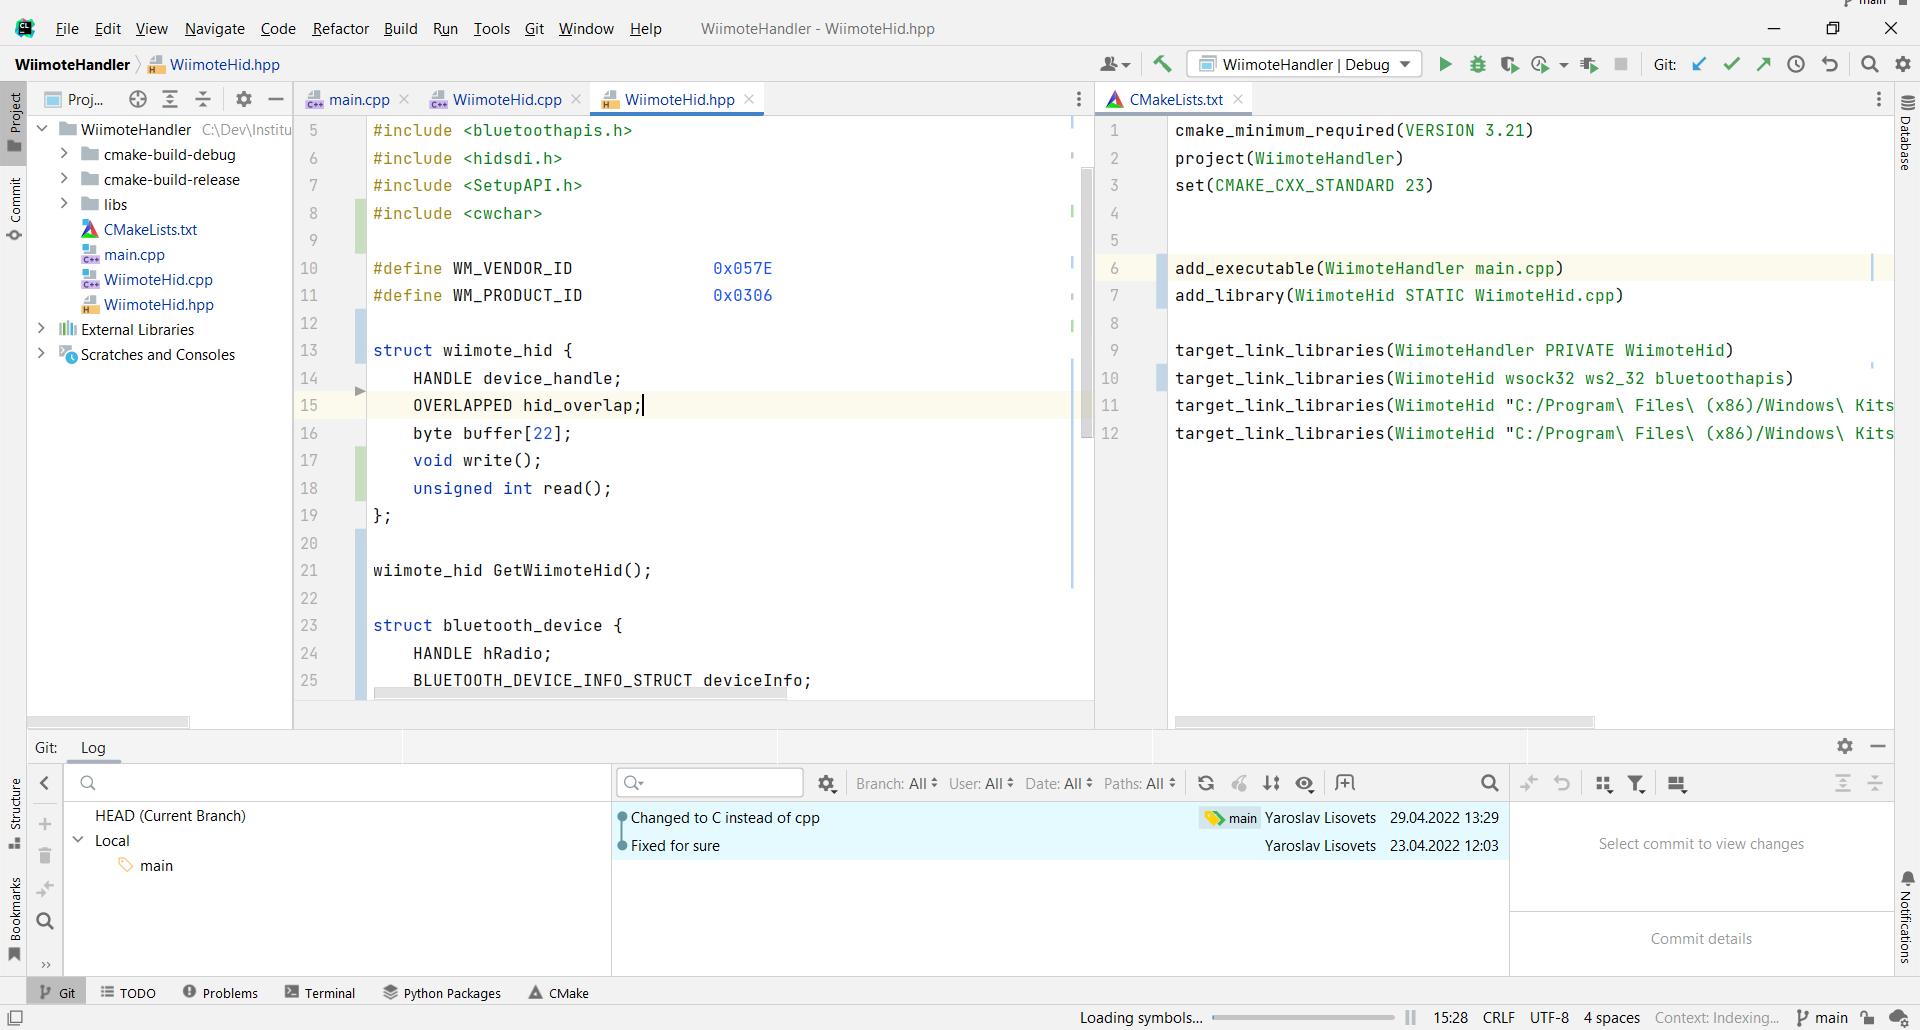
\includegraphics[width=\textwidth]{content/clion_screenshot}
\captionof{figure}{Скриншот из Clion с открытыми окнами редактирования заголовочного файла и файла CMake }

\subsubsection{IntelliJ Rust}
\quad IntelliJ Rust\footnote{плагин с открытым исходным кодом совместимый со всеми IDE основанными на IntelliJ IDEA для Rust.\href{ https://plugins.jetbrains.com/plugin/8182-rust}{https://plugins.jetbrains.com/plugin/8182-rust}}
- плагин с открытым исходным кодом совместимый со всеми IDE основанными на IntelliJ IDEA\@.
В паре с IntelliJ TOML  \footnote{IntelliJ TOML \href{ https://plugins.jetbrains.com/plugin/8195-toml}{https://plugins.jetbrains.com/plugin/8195-toml}} он направлен на то, чтобы привнести полный опыт IDE в ваш рабочий процесс с Rust и Cargo.

\subsubsection{CMake}
\quad \text{CMake\footnote{Семейство инструментов CMake \href{https://cmake.org/}{https://cmake.org/}}
 - это семейство} инструментов с открытым исходным кодом для создания, тестирования программного обеспечения.
 CMake используется для управления процессом компиляции программного обеспечения с помощью простых файлов конфигурации,
 независимых от платформы и компилятора.